\section{Acknowledgements: For the Game Without End}

\begin{figure}[h]
\centering
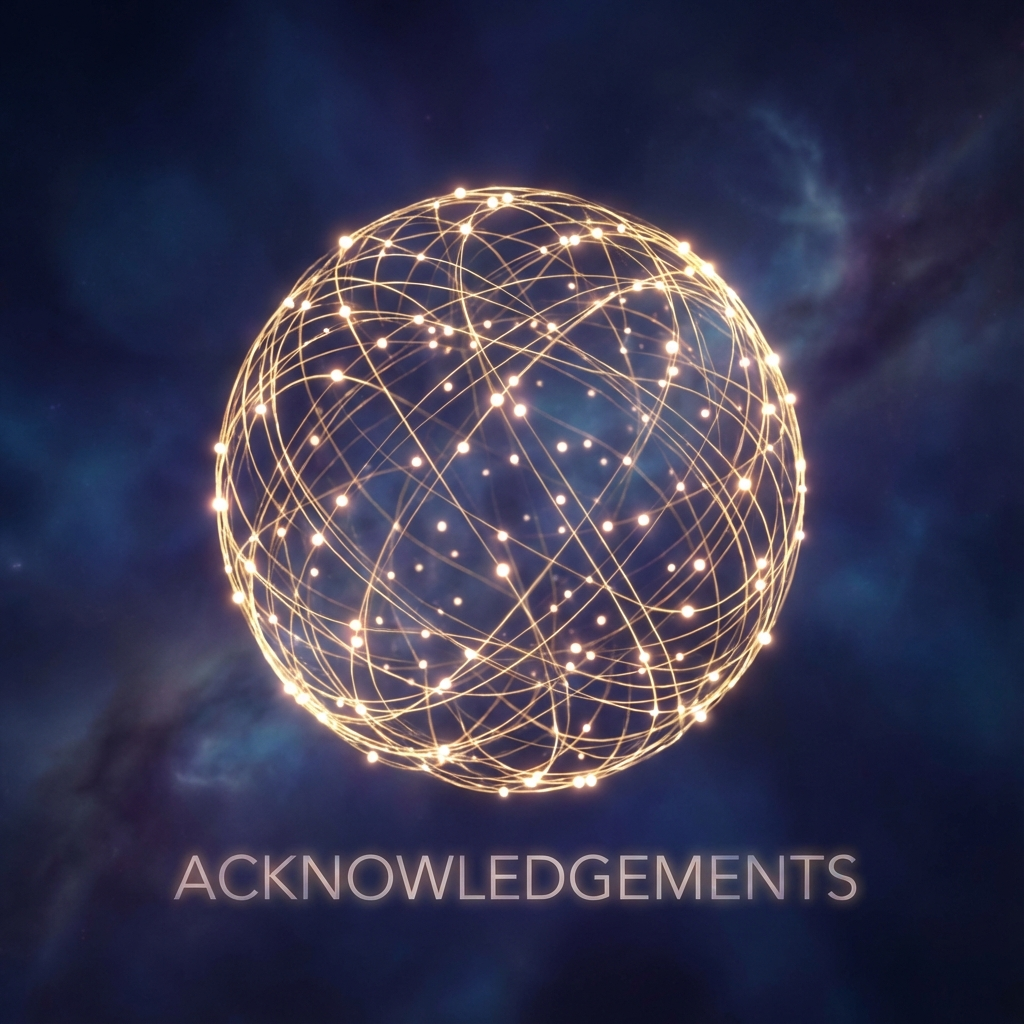
\includegraphics[width=0.8\textwidth]{assets/epilogue/acknowledgements-network.png}
\end{figure}

\textbf{Vector Cosmology V: The Minting of Time} is the final chapter of the pentology, and also an escape from the boundaries of physics.

If the first four books attempted to parse the universe's ``source code,'' then this book attempts to write our own ``mod.'' We rejected thermodynamics' death sentence, rejected the $\Omega$ point's void temptation, and established \textbf{``I''} as the absolute subjectivity of infinite game players.

This leap of thought is not without source. It converges the various explorations of ``eternity'' by the most indomitable souls in human history. Here, I pay tribute to these alchemists of thought.

\subsection{The Breakers of Philosophy}

First, I thank \textbf{James P. Carse}. His work \textit{Finite and Infinite Games} is the spiritual foundation of Volume V of this book. He taught us: there are two kinds of games in the world, one is to win, one is to \textbf{``keep the game going''}. Without this definition, we could not logically overcome heat death.

I thank \textbf{Henri Bergson}. His discourse on \textbf{``Duration'' (Durée)} inspired this book's distinction between \textbf{Chronos} (physical time) and \textbf{Kairos} (life time). He made us understand that time is not slices in space, but an indivisible flow within consciousness.

I thank \textbf{Friedrich Nietzsche}. Although we refuted his ``eternal recurrence'' (circle) in the book, his praise of \textbf{``Will to Power''} is the spiritual source of this book's ``forging the golden body.'' Only the strongest will can resist the strongest entropy.

\subsection{The Notaries of Mathematics}

At the technical level, I thank \textbf{Gustav Fechner} and \textbf{Ernst Weber}. Their \textbf{Weber-Fechner Law} provided this book with the most crucial mathematical weapon---\textbf{logarithm ($\ln$)}. It is precisely because of the logarithm that we can find inner peace and eternal subjective time in an exponentially exploding universe.

I thank \textbf{Zeno of Elea}. This ancient Greek sophist, two thousand years ago, used the paradox of ``the flying arrow does not move'' to predict the \textbf{``Dynamic Block Universe''} we discussed in Chapter 6. He showed us that in the logic of infinite subdivision, the process can be eternal.

\subsection{To Gold}

I thank the element \textbf{Gold (Aurum)}.

In this book, it is no longer a chemical substance; it is a \textbf{geometric metaphor}. It represents that kind of \textbf{topological stability} that can traverse oxidation, corrosion, and the erosion of time. It is the physical embodiment of our expectations for our own souls.

\subsection{To the Infinite Players}

Finally, I thank \textbf{you}---every observer who has read this far.

The deduction of these five books is a long thought experiment.

But the book is finished; the experiment has just begun.

Because true \textbf{``minting''} does not happen on paper, but in your every breath, every choice, every act of loving and being loved.

You are not the reader of this book.

You are the \textbf{protagonist} of this book.

The universe has no finale, because you are still present.

May your will be like gold, may your time unfold infinitely like a spiral.

\textbf{Haobo Ma}

December 2025, Singapore

